\chapter{基于优化CPU和GPU内存交互的设计和实现}
前两章总结了大数据高通量仿真中CPU/GPU异构并行计算的必要性和一些已有的GPU异构编程优化方法,并利用编译
原理中引用-定值链和定值-引用链分析程序中的数据流,介绍了一些适用于一般程序的代码移动优化方法。
程序员只有清楚的了解CPU/GPU的体系结构特点,再根据具体的应用场景设计合适的程序逻辑,选择合适的GPU编程
优化方法才能够编写出充分利用GPU计算性能的程序。本章基于CPU/GPU异构计算的内存隔离特点,结合编译原理中的代码
移动规则新提出了一种通过修改源代码来减少CPU和GPU内存之间数据交换带来的系统消耗的优化方法,并在第四章
通过一些对比实验证明了本文提出的方法确实有优化GPU程序的作用。
\section{迁移数据交换操作}
由于CPU和GPU的内部结构不同,CPU适合处理顺序计算、程序逻辑以及系统IO等任务,而GPU适合处理高度并行的复杂计算任务。
所以在CPU/GPU异构体系结构中运行的程序包含CPU代码、GPU代码以及CPU和GPU的交互代码。
普通的程序逻辑就是CPU代码,CPU和GPU内存之间的数据交换操作就是交互代码,核函数就是由GPU代码组成的。
CPU内存和GPU内存是隔离的,运行CPU代码时我们把需要的所有数据拷贝到GPU内存中,同样地运行GPU代码时,我们需要把所有数据拷贝
到GPU内存中。所以GPU程序中每一次核函数的调用,通常会在CPU内存和GPU内存之间进行两次数据交换。核函数执行之前,
CPU和GPU执行相应的交互代码API(CudaMalloc、CudaMemcpy)在GPU内存分配相应大小空间并把核函数需要的数据拷贝到GPU已分配
内存中,这个过程称为数据拷入操作(data copyin)。data copyin操作结束之后,GPU开始启动运行核函数(execution)。
在核函数计算结束之后,我们需要把GPU中计算的结果再次拷贝到CPU内存,称为数据拷出(data copyout)。最后如果GPU
中的变量不会再被后续核函数使用,GPU会释放核函数运行之前分配的GPU内存,这是数据释放操作(data freeing)。
由此可见数据在CPU和GPU内存交换的总时间是由一下三个部分组成的:1.在GPU内存上分配空间等预处理操作时间;
2.数据在PCIe总线上传输时间;3.GPU释放内存等清理操作时间。在核函数比较多的程序中,CPU和GPU之间频繁的数据交换
将成为整个程序的瓶颈,这也是本文优化方法的出发点。本节主要是根据编译原理中代码移动原理迁移GPU程序中核函数的数
据拷贝操作,使原来在程序中固定点执行的数据交换操作可以允许在程序中的一段代码区间执行。
\subsection{迁移限制}
如上所述,一个核函数的执行被拆分成了四个独立的阶段,数据拷入, 执行, 数据拷出和数据释放。
显然这四个阶段的执行顺序是不能颠倒的,必须按照数据拷入$\rightarrow$执行$\rightarrow$数据拷出$\rightarrow$数据释放
的顺序执行,但是每个操作具体的执行时间确是可以调整的。本文的出发点是优化数据交换操作,所以我们不迁移核函数的执行
操作,只迁移数据拷入,数据拷出,数据释放三个数据交换操作。我们可以把数据拷入操作的交互代码可以看作是CPU代码中对变量的一个引用,可以沿着
代码语句序列向上移动直到程序中某个点改变了该数据,即遇到该变量的定值点就不能再向上移动了,同时我们得保证数据拷入操作
在核函数开始执行之前完成。同样地,我们也可以把交互代码中的数据拷出操作看作是CPU代码中队变量的定值,可以和数据释放操作一起
沿着代码语句序列向下移动,直到程序中出现某条语句引用该变量,即遇到该变量的引用点结束,同时我们必须保证数据
拷出和数据释放操作是在核函数执行完成之后才开始执行的。数据拷出操作之后,为了减少GPU内存的占用,我们将立刻释放相应的GPU内存,
除非该内存数据会在后续的核函数中继续用到我们才选择继续保存,这样可以减少冗余的数据拷贝。
所以在整个数据交换操作的迁移过程中数据依赖性是迁移的前提,
在下面的章节我们将利用编译原理中的引用-定值链和定值-引用链方法来分析
整个程序中的控制流和数据流,得到具体的迁移操作。
\subsection{代码移动}
现在我们介绍如何调整核函数执行过程中的四个阶段,以及如何根据代码移动方法迁移核函数的数据交换操作。
代码块~\ref{Listing4}描述了原始CUDA代码中一个核函数的结构,数据拷入操作,核函数执行,数据拷出操作,以及数据释放操作
是一个紧密的整体。但是在代码块~\ref{Listing5}中,数据拷入操作被提前执行,同时数据拷出和数据释放操作被推后执行。
显然代码块~\ref{Listing5}中针对数据操作的迁移并没有改变代码块~\ref{Listing4}中的执行结果。
本文的GPU程序优化算法只针对CPU和GPU内存之间的数据交换操作,所以我们只迁移数据交换操作。
\newpage
\begin{lstlisting}[label=Listing4,caption=原始CUDA代码,language=C, keywordstyle=\color{blue!70},commentstyle=\color{red!50!green!50!blue!50},frame=shadowbox, rulesepcolor=\color{red!20!green!20!blue!20}] 
__global__ void kernel(int *device, int i);
int host[1000] = {0}, tmp[1000] = {0};
for (int i = 0; i < 1000; i++)
    host[i] = host[i] + 1;
......
for (int i = 0; i < 1000; i++)
    tmp[i] = tmp[i]+1;
int *device;
CUDAMalloc(&device, sizeof(int) * 1000);
CUDAMemcpy(device, host, sizeof(int) * 1000,CUDAMemcpyHostToDevice); /*data copyin*/
for (int i = 0; i < 1000; i++) /*execution*/
    kernel<<<1,1>>>(device, i);
CUDAMemcpy(host, device, sizeof(int)* 1000,
CUDAMemcpyDeviceToHost); /*data copyout*/
CUDAFree(device); /*data freeing*/
......
for (int i = 0; i < 1000; i++)
    tmp[i] = tmp[i]+1;
\end{lstlisting}

\begin{lstlisting}[label=Listing5,caption=迁移数据拷贝操作,language=C, keywordstyle=\color{blue!70},commentstyle=\color{red!50!green!50!blue!50},frame=shadowbox, rulesepcolor=\color{red!20!green!20!blue!20}] 
__global__ void kernel(int *device, int i);
int host[1000] = {0}, tmp[1000] = {0};
for (int i = 0; i < 1000; i++)
    host[i] = host[i]+1;
int *device;
CUDAMalloc(&device, sizeof(int) * 1000);
CUDAMemcpy(device, host, sizeof(int) * 1000, CUDAMemcpyHostToDevice); /*data copyin*/
......
for (int i = 0; i < 1000; i++)
    tmp[i] = tmp[i]+1;
for (int i = 0; i < 1000; i++) /*execution*/
    kernel<<<1,1>>>(device, i);
......
for (int i = 0; i < 1000; i++)
    tmp[i] = tmp[i]+1;
CUDAMemcpy(host, device, sizeof(int)* 1000,
CUDAMemcpyDeviceToHost); /*data copyout*/
CUDAFree(device); /*data freeing*/
\end{lstlisting}
核函数的数据拷入操作可以沿着代码语句序列向上移动,我们只要保证数据拷入操作在相应数据的定值点之后和核函数执行之前的代码区间执行就是合法的。
同样数据拷出操作可以沿着代码语句序列向下移动,我们只要保证数据拷出操作在相应数据的引用点之前和核函数执行之后的代码区间执行就是合法的
至于核函数的数据释放操作,必须保证在数据拷贝操作之后执行。当程序在GPU上内存使用量较少而且GPU内存足够使用时,我们可以选择让GPU内存保持所有的
数据直到整个程序执行结束之后释放。但是GPU内存在使用时不总是足够的,所以我们选择在数据拷出到CPU内存之后立刻让GPU内存释放该变量,除非该变量
在后续核函数中会再次用到才让GPU内存保持。
\subsection{异步操作优化}
\begin{figure}[h]
\centering
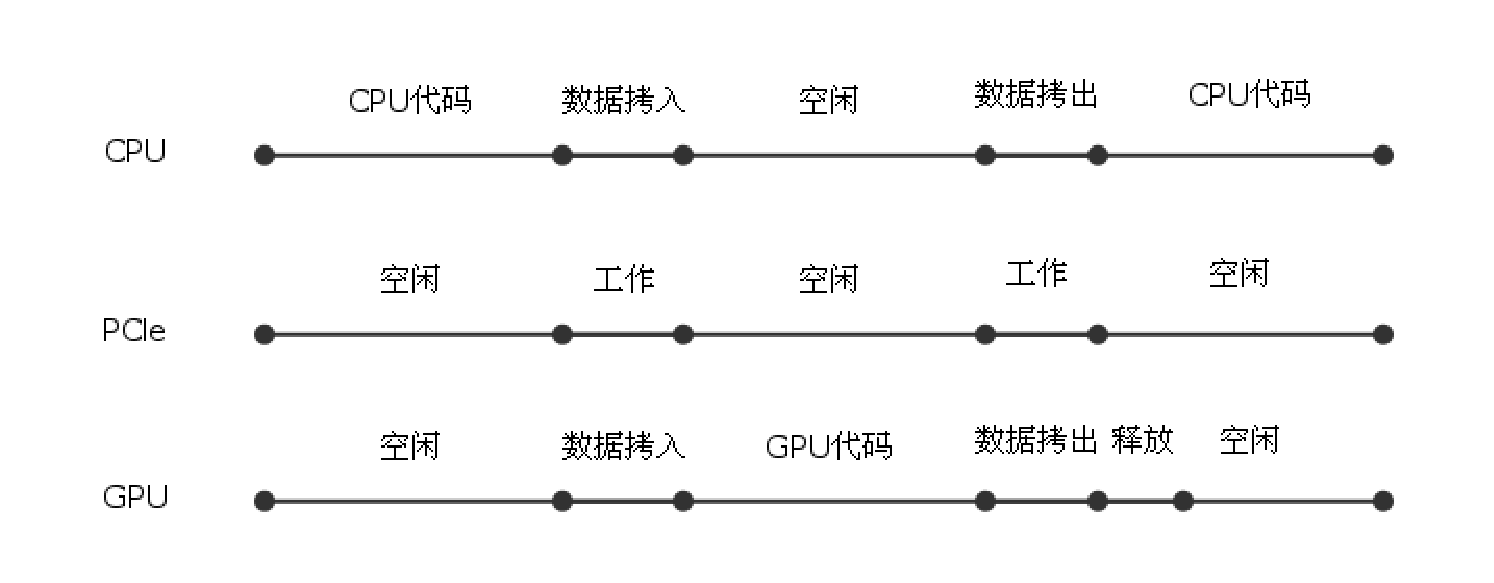
\includegraphics[width=1\linewidth]{figure9.eps}
\caption{初始结构}\label{figure9}
\end{figure}
\begin{figure}[h]
\centering
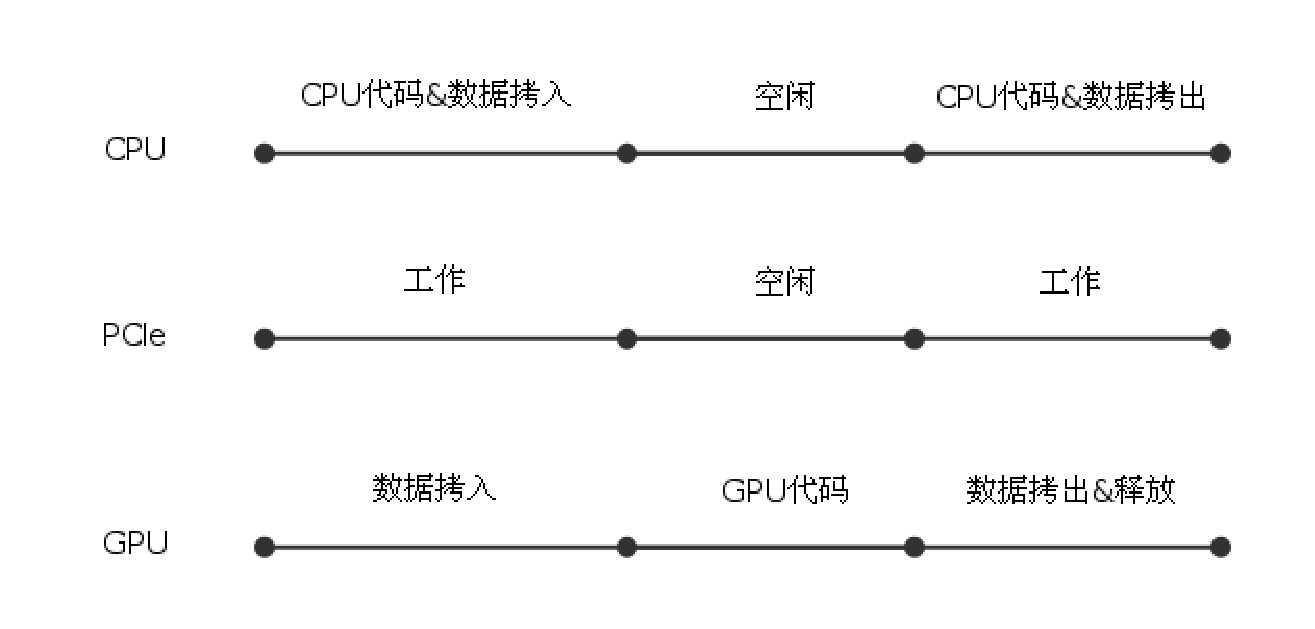
\includegraphics[width=1\linewidth]{figure10.eps}
\caption{异步优化}\label{figure10}
\end{figure}
这里先单独讨论一下单个核函数在数据拷贝操作迁移之后的异步优化。我们发现数据拷入操作沿着代码序列向上移动之后,数据拷入操作和核函数执行的代码语句之间
出现了一部分CPU代码。同样地,数据拷出操作沿着语句序列向下移动之后,核函数结束执行和数据拷出操作之间也有一部分CPU代码。我们再迁移数据交换操作时是以
数据依赖性为前提的,所以这部分CPU代码和数据交换操作时没有任何依赖的,即可以异步并行执行。图~\ref{figure10}对图~\ref{figure9}中单个核函数的
执行过程进行了一些异步优化。首先在图~\ref{figure9}中第一段CPU代码执行时,PCIe和GPU都处于空闲状态,数据拷入操作在CPU代码完全执行结束之后才开始。
我们在代码块~\ref{Listing5}中可以看到,在迁移数据拷入操作之后,又一块CPU代码可以和数据拷入操作异步执行。CPU代码执行时不占用PCIe总线和GPU资源,
GPU预分配内存和数据拷入操作也不占用CPU代码执行时需要的计算资源。图~\ref{figure10}中的并行策略可以更加充分地利用CPU/GPU资源和PCIe总线带宽。
同样地,我们也可以对数据拷出操作和CPU代码进行异步优化,这里就不做赘述。
当然如果程序员足够聪明,可以在设计核函数时就选择以异步的方式进行数据拷贝操作。
异步优化必须要有一块与数据交换操作无依赖、可并行的CPU代码时才能发挥作用,这与我们本文提出的减少数据交换频率和数据交换总量的优化方法不相同。



